\documentclass{article}

\usepackage{listings}
\usepackage{color}
\usepackage{graphicx}
\usepackage{float}
\usepackage{amsmath}
\usepackage{subfig}

\begin{document}

\title{$\mu$Image Manipulator}

\author{Hamid Mirisaee,
\and Jander Nascimento, 
\and Raquel Oliveira}

\maketitle

\tableofcontents

\section{Filters}

	\subsection{Fundamental}

		By definition, a filter is a device or process which removes some unwanted features from an image (more precisely, form a signal).
		low-pass and high-pass filters are regarded as a classic example of filters in image processing field. Generally, filters are used to be convolved 
		(the convolution is described in the next part) with an image in order to produce a new, modified image. This new image, in turn, could
		be used for some other processings. The next subsection will introduce the convolution and its basics.
		
		\subsubsection{Convolution}

			Convolutions are used to perform many useful image processing tasks such as noise reduction and edge detection. Generally,
			convolution is a mathematical operation on two functions f and g to produce a modified version of one of the functions.
			Generally, but not necessarily, the first function (signal) is the input and is bigger than the second one.
			The following formulas describe the discrete convolution formula in 1D and 2D space:


			\[y[n] = f[n]*g[n] = \sum_{k=-\infty}^{+\infty} f[k]g[n-k]\]

			\[y[m,n] = f[m,n]*g[m,n] = \sum_{i=-\infty}^{+\infty}\sum_{j=-\infty}^{+\infty}f[i,j]g[m-i,n-j]\]


			
			When dealing with finite-length sequences, one cannot use the ordinary convolution formula (called linear convolution).
			In such cases, the circular convolution which results in zeros outside of the range of the signal is used. The mathematical formula of discrete 
			convolution could be seen in the following:

			\[y[n] = f[n]*g[n] = \sum_{k=-K/2}^{+K/2} f[k]g[n-k]\]

			\[y[m,n] = f[m,n]*g[m,n] = \sum_{i=-K/2}^{+K/2}\sum_{j=-T/2}^{+T/2}f[i,j]g[m-i,n-j]\]



			
			
			In image processing field, generally, the input image is the first function of the convolution, and the second 
			function is considered as the kernel or filter.
			In this context we use the terms kernel and filter interchangeably.
			There is a wide range of filters which are used to perform different tasks on a given image. The next subsection would go through some of these 
			filters which are used in the application in addition to a brief description for each of them.

		\subsection{Used filters}
		
		\subsubsection{Gaussian}

			The Gaussian kernel is a 2D convolution operator which is used to blur an image and remove noise. Mostly, applying a convolution using a Gaussian
			kernel is called Gaussioan smoothing.Generally, the Gaussian kernel is centered at
			zero (pick at 0). The following describes the Gaussian formula in 2D space:

			\[G(x,y) = \frac{1}{2\pi\sigma^{2}}e^{-\frac{x^{2}+y^{2}}{2\sigma^{2}}}\]

			
			Gaussian smoothing acts almost the same as the mean filter, which will be in the following part.
		\subsubsection{Mean}
			Mean filter is an easy to implement kernel which is used to reduce the noise in an image by reducing the amount of intensity variation between one
			pixel and the next. The idea of the mean filter is to replace the value of each pixel with the average of its neighbors including itself. As an example,
			a 3*3 mean filter is a matrix in which all cells filled up with 1/9 .	
		
		\subsubsection{Gradient}

			Applying gradient filter to an image is one of the edge detection approaches. Before explaining the gradient filter and its properties, we will see
			short description of edge detection concept. 
			
			Technically, an edge is a part of image where a sharp change is occurred in the brightness of the pixels.
			More informally, edges are the boundaries of
			the objects in an image. Detecting edges in an image is a non-avoidable issue in some image processing tasks such as intelligent resizing.
			
			Mathematically, gradient is the first derivation of the image. In other words, it is a vector with a certain magnitude and direction. 
			The magnitude of the gradient provides information about strength
			of the edge, and the direction of the gradient is always perpendicular to the direction of the edge. Clearly, the gradient filter could be
			applied horizontally and vertically. The gradient vector is given below:

			There are several filter based on gradient concept. Sobel edge detector and Prewitt edge detector are two well-known filters.
			As it is mentioned previously, gradient approach is based on the first derivation of the input. Based on the properties of
			the first derivation, the edges of a given input could be seen near the picks in the first derivation curve. Accordingly, a threshold should be
			determined in order for the edges to be detected. However, since a thresholding is used, the edges might be too thick to be considered
			as an edge. As a result, we may need to apply a localization method (for instance, using Laplacian filter) to find zero
			crossing points and separate actual edges from other non-edge points. The following illustrates the Prewitt operator in x-direction. The y-direction, clearly, is the transpose of the x-direction.


\begin{figure}[H]
\begin{center}
 \begin{tabular}{ | l | c | r | }
    \hline
    -1 & 0 & 1 \\ \hline
    -1 & 0 & 1 \\ \hline
    -1 & 0 & 1 \\
    \hline
  \end{tabular}
\end{center}
\caption{Prewitt operator in x-direction}\end{figure}

		
		\subsubsection{Laplacian}
			The Laplacian filter is computed based on the second derivation of the input. The following matrix is an approximation of a 3*3 Laplacian filter; however, a 5*5 filter is used in the developed application based on better results it resulted in for
most of the tested images.

\begin{figure}[H]
	\begin{center}
  \begin{tabular}{ | l | c | r | }
    \hline
    -1 & -1 & -1 \\ \hline
    -1 & 8 & -1 \\ \hline
    -1 & -1 & -1 \\
    \hline
  \end{tabular}
\end{center}
\caption{an example of a 3 by 3 Laplacian filter}\end{figure}


			 As a result, it is highly sensitive to noise. Consequently,
			it is generally applied after noise reduction filters. Alternatively, one can use LoG (Laplacian of Gaussian) since the convolution is
			associative. The following is the LoG formula in 2D space:

			\[LoG(x,y) = -\frac{1}{\pi\sigma^{4}}[1-\frac{x^{2}+y^{2}}{2\sigma^{2}}]e^{-\frac{x^{2}+y^{2}}{2\sigma^{2}}}\]

			

\section{Color space}    
	A color model is a model by which the color are represented by a few numbers, typically three or four. Using primary colors, a vast variety of colors could be made. Two well-known models are RGB and CYMK.      

	\subsection{RGB}
		In RGB model red, green and blue lights areadded together to make a wide range of colors. This model is generally used in electronic systems such as CRTs and LCDs. In case of an 8-bit value for each color, more than 16 million different colors
		could be made using this model. The RGB model is considered as an additive model, which means the white color is a result of combination of all lights while black is a result of absence of all the lights.
	

	\subsection{CYMK}

		CMYK (Cyan, Magenta, Yellow, Key black) is another color model which is used in color printing. Unlike the RGB, CMYK is a subtractive; that is, white is is the natural color of the paperand black is a full mixture of all colors.
		As a result, to save money on ink, the dark colors and the blac is produced using the black ink.

	\subsection{Gray scale conversion}

		In order to conver an image to gray scale from an RGB image, we need to consider that how far a pixel is from black. To achieve this goal, one can substitue all the colors of a pixel with the average of the three colors. Using
		this method, a pure black pixel would remain black, and a white pixel would still remain white. Other pixels, however, would be have a gray view between black and white.

\section{Cropping}

	Cropping is a technique where the main purpose is to change or improve the visibility of a certain object in an image, 
	this is done by removing external frames. 

	The new target becomes the main object of the image generating a new image with the dimension of the target area.  

	\begin{figure}[H]
	  \centering
	  \subfloat[Non cropped image]{\label{fig:nonnormalized}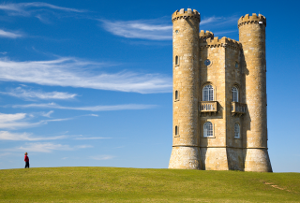
\includegraphics[width=0.3\textwidth]{images/crop_1}}                
	  \subfloat[Cropped image]{\label{fig:normalized}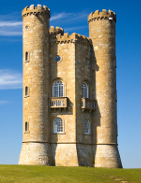
\includegraphics[width=0.3\textwidth]{images/crop_2}}
	  \caption{Image cropping}
	  \label{fig:cropping}
	\end{figure}


\section{Fusion}

	\textit{Fill me}.

\section{Resizing}

	Image resizing consist in convert an image to a size in which may or not respect the previous ratio.
	When dealing with reducing the size of an image is quite simple to do it, but when dealing with enlarging 
	the image, the process is a little bit complex.

	Reducing the dimension of an image consist in removing as many lines and as many columns as necessary to reach target dimension, of course this
	process may create some side-effect in the image, 

	When we stretch an image, we have few known pixels (dots which are image composition, think like the cells of a human being).

	There is a lot of algorithms that helps to guess (fill the gaps) those unknown pixels. for instance:

	\begin{itemize}
	  \item Nearest neighbor interpolation
	  \item Linear interpolation
	  \item Bilinear interpolation
	  \item Bicubic interpolation
	\end{itemize}

	The adopted algorithm is, \textbf{Bilinear interpolation},  due its speed and simplicity.
	
\subsection{From Linear to Bilinear interpolation}

	The Linear interpolation may be done horizontally or vertically, or even both. If a horizontal or vertical interpolation is done, we call it
	Linear interpolation, case both interpolations are applied its called Bilinear interpolation.	
	The pixel interpolation is done by calculating the mean of the known pixels around (vertical and horizontal axis) the unknown pixel. 

	\begin{figure} [H]
		\centering
		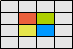
\includegraphics[scale=1]{images/bilinear_interpolation_1}
		\caption{original image \label{bilinear1}}
	\end{figure}

	On \ref{bilinear1} we can see the original image where all pixel are known pixels. Now what happen if we stretch this image 
	from a 2x2 to a 3x3 image?
	
	\begin{figure} [H]
		\centering
		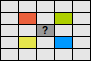
\includegraphics[scale=1]{images/bilinear_interpolation_2}
		\caption{image resized from 2x2 to 3x3 \label{bilinear2}}
	\end{figure}

	As we can see, after stretch the image to a desired dimension we create some unknown pixels. To those pixels we can apply the linear interpolation 
	to guess the color intensity we should use based in the color of it's neighbor pixels (not by simply copying the neighbor).

	Example above is not realistic, for several reasons. First of them is that in most of the cases we must fill more than one gap in between known pixels,
	second is that in real cases we consider the pixel in the horizontal and vertical direction, instead of diagonal axis. Third reason is that in the 
	previous example the distance between the unknown pixel to the known pixel were always the same, so a regular division would. 
	Check this other example, a bit more realistic:
	
	\begin{figure} [H]
		\centering
		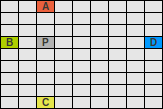
\includegraphics[scale=1]{images/bilinear_interpolation_3}
		\caption{more realistic image\label{bilinear3}}
	\end{figure}
	
	In the example above we can see that the interpolation cannot be only the mean of the pixel, since the unknown pixel 
	is closer to the point A and B, it's reasonable 
	this unknown pixel receives A and B color than the other ones.

	Consider \textit{distance(p1,p2)} a function that returns the distance between two pixels, 
	and \textit{color(p1)} a function that returns the color of the pixel p1 . We perform first the Linear interpolation horizontally, so:

	\[ f_h(p)=color(B)*\frac{distance(P,D)}{distance(B,D)}+color(D)*\frac{distance(B,P)}{distance(B,D)}  \]

	We can perform this operation in the vertical axis as well:

	\[ f_v(p)=color(A)*\frac{distance(P,C)}{distance(A,C)}+color(C)*\frac{distance(A,P)}{distance(A,C)}  \]

	Combibing these two approaches we have the bilinear interpolation.

	
\section{Histogram}

	\subsection{Color histogram}

		The histogram is an important tools when dealing with image analysis. It shows the color distribuition of a certain image regarding to its 
		color \textit{spectrum}.
			
		The histogram is represented in a cartesian, where \textit{x} axis is the 
		color \textit{spectrum} and \textit{y} represents the number of pixels.

		In colorful images, histogram instead of representing the color \textit{spectrum} of a single color we may use two techniques
		to represent colorful images, either by summing all the colors into a single histogram, or create a differente histogram for each 
		color.
		

	\subsection{Normalization}
		
		The normalization, or histogram stretching, is a technique where the color histogram is used to evaluate and possible change
		the color intensity range. This, enhances the detail level of some images that might appear too dark or too light (duo to aperture size of even
		bad light condition).

		This is done by spreading the pixels to use as much as possible the entire color \textit{spectrum}.
		
		\begin{figure}
		  \centering
		  \subfloat[Un-normalized]{\label{fig:nonnormalized}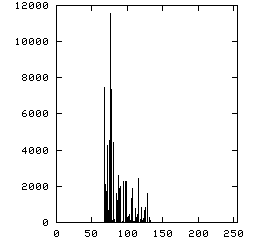
\includegraphics[width=0.3\textwidth]{images/histogram_1}}                
		  \subfloat[Normalized]{\label{fig:normalized}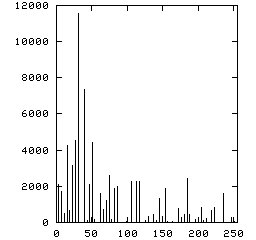
\includegraphics[width=0.3\textwidth]{images/histogram_2}}
		  \caption{Histogram normalization}
		  \label{fig:normalization}
		\end{figure}

		

		To perform the normalization, the only variables we must know to perform this operation is the minimum and maximum color in the current histogram, 
		and minimum and maximum color in the enhanced histogram, or we may translate as a new position for the minimum and maximum colors. It is possible
		to write mathematically the formula \ref{eq:normalization}.


		\begin{equation}
			normalize(p)=new_{min}+\frac{new_{max}-new_{min}}{current_{max}-current_{min}}*(p-current_{min})
			\label{eq:normalization}
		\end{equation}
		
		
\section{Supported image formats}


		\begin{center}
		    \begin{tabular}{ | l | l |}
		    \hline
		    	PNG & Windows Bitmap \\ \hline
			PNG & Portable Network Graphics\\ \hline
			PBM & Portable Bitmap\\ \hline
			PGM & Portable Graymap\\ \hline
			PPM & Portable Pixmap\\ \hline
			TIFF & Tagged Image File Format\\ \hline
			XBM & X11 Bitmap\\ \hline
			XPM & X11 Pixmap\\ \hline
			SVG & Scalable Vector Graphics\\ \hline
		    \end{tabular}
\end{center}

\end{document}
